\section{Presupuesto}

En este apartado se detalla el presupuesto estimado necesario para desplegar el sistema propuesto. La estimación final del presupuesto será el costo total a duración de un año.

\subsection{Infraestructura Web}

El coste de la infraestructura se fracciona en 2 partes, el dominio y el servidor a alquilar.

\subsubsection{Dominio}

El coste actual de los dominios varia dependiendo del proveedor y de la extensión que se desee contratar. Para este trabajo, el dominio que se desea contratar es \quotes{uacrowdfunder.com}, con el proveedor Namecheap\footnote{www.namecheap.com}.

\bigskip

El costo estimado del dominio con Namecheap es de 8,76eur / Año.

\begin{figure}[H]
        \centering
        
\includegraphics[width=1\textwidth]{img/capturas/dominio.png}
        \caption{Presupuesto - Coste anual del dominio.}
        \label{fig:configApi}
\end{figure}

\newpage

\subsubsection{Alojamiento Web}

Para el alojamiento de la página web en cuestión, existen diversas alternativas. En este caso, la aplicación front-end se encuentra completamente encapsulada en una imagen docker, lo que permite considerar tres opciones: la utilización de un servidor privado virtual con docker instalado, el uso de un servicio de alojamiento de contenedores autogestionado, o la elección de un servicio de alojamiento de páginas web, evitando así la necesidad de utilizar docker. 

\bigskip

Para el propósito de este trabajo, se opta por un VPS por conveniencia para el desarrollador. Al emplear un VPS, el único pago a gestionar es el correspondiente al servidor. Los precios por este tipo de servicios suelen variar dependiendo del proveedor, pero a diferencia de otros servicios, el costo es único, y no fluctúa en función del uso de los recursos del servidor.

\bigskip

En este caso, se ha contratado un VPS con el proveedor Contabo\footnote{www.contabo.com}, que ofrece recursos más que suficientes para el despliegue de la aplicación web

\bigskip

\begin{figure}[H]
        \centering
        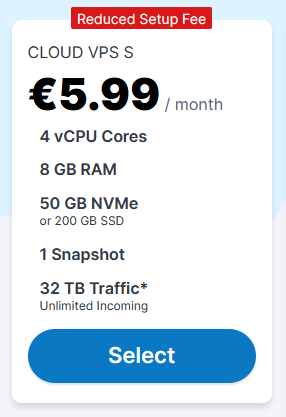
\includegraphics[width=0.4\textwidth]{img/capturas/vps.png}
        \caption{Presupuesto - Coste mensual del VPS.}
        \label{fig:configApi}
\end{figure}

Este plan tiene un coste único de instalación de 4eur, y un coste mensual de 6eur / mes.

\newpage

\subsection{Smart Contract}

El coste del smart contract varia dependiendo del precio actual del gas y de la red que se usa. Para ello, los costes usado para esta estimación serán de la fecha actual (14:20 - 21/04/2023) en la red Polygon.

\subsubsection{Despliegue}

El coste asociado al despliegue se incurre una única vez durante la publicación del smart contract en la blockchain y está condicionado por la densidad del contrato. 

\bigskip

Por otro lado, el coste de cada función se estima en gas, variando según el coste computacional de cada método del contrato. En este contexto, únicamente se toma en cuenta como parte del coste el despliegue del contrato, dado que el coste del gas utilizado por los métodos será asumido por los usuarios de la plataforma.

\bigskip

Considerando que el contrato desarrollado no cumple con todos los requisitos de la plataforma, para la estimación se duplicará el coste del despliegue de este contrato, proporcionando así una cota superior pesimista del coste real que podría implicar el despliegue de un contrato con todas las funcionalidades implementadas. 

\bigskip

Para determinar el coste del despliegue en la Mainnet de Polygon, se recurre al estimador de MetaMask. Durante el despliegue del contrato, se puede observar el coste en Euro del despliegue del contrato en la red.

\bigskip

\begin{figure}[H]
        \centering
        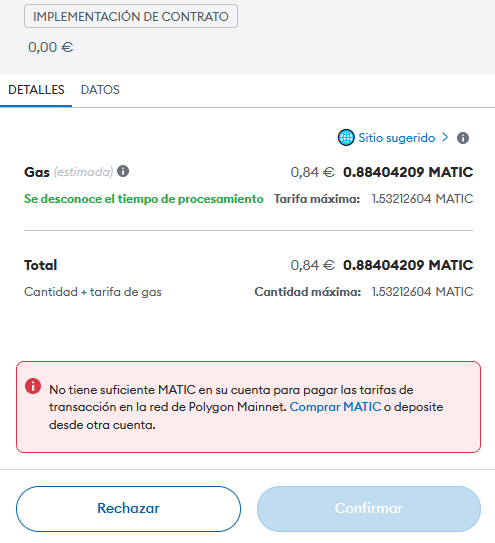
\includegraphics[width=0.4\textwidth]{img/capturas/contractcost.png}
        \caption{Presupuesto - Coste del despliegue del contrato en Euro.}
        \label{fig:configApi}
\end{figure}

La captura revela el gas requerido para realizar la transacción y el coste equivalente en Euro, representando un pago único de un total de 0,84 Eur. Dado que el despliegue se refiere al contrato de la prueba de concepto, al duplicar dicho coste se obtiene una estimación de 1.68 Eur.

\newpage

\subsection{Tabla de totales}

A continuación se muestra una tabla con los costes totales del mantenimiento y despliegue del sistema a plazo de un año.

\begin{table}[h!]
\centering
\label{tab:costes}
\begin{tabular}{@{}l S S S@{}}
    \hline
    \textbf{Concepto} & \textbf{Coste único (EUR)} & \textbf{Coste mensual (EUR)} & \textbf{Coste anual (EUR)} \\ 
    \hline
    Dominio & 0 & 0 & 8.76 \\
    Alojamiento VPS & 4 & 6 & {6*12} \\
    Despliegue Smart Contract & 1.68 & 0 & 0 \\ 
    \hline
    \textbf{Total} & \textbf{5.68} & \textbf{6} & \textbf{80.76 Eur} \\ 
    \hline
\end{tabular}
\caption{Presupuesto - Tabla de totales.}
\label{tab:tablatotales}
\end{table}
